% === Revtex Declaration ===
\documentclass[aps, 10pt, english, twoside, pra, nofootinbib, tightenlines, longbibliography, superscriptaddress, notitlepage]{revtex4-1}

% === Bibliography Style Options ===
\bibliographystyle{apsrev4-1}
\setlength{\bibsep}{3pt plus 3pt minus 2pt}

% === Packages ===
\usepackage{document_config}

\begin{document}
    \title{Erratum: Causal Compatibility Inequalities Admitting Quantum Violations in the Triangle Structure}
    \author{Thomas C. Fraser}
    \email{tfraser@perimeterinstitute.ca}
    \affiliation{Perimeter Institute for Theoretical Physics, Waterloo, Ontario, Canada, N2L 2Y5}
    \affiliation{University of Waterloo, Waterloo, Ontario, Canada, N2L 3G1}
    \author{Elie Wolfe}
    \affiliation{Perimeter Institute for Theoretical Physics, Waterloo, Ontario, Canada, N2L 2Y5}
    % \email{ewolfe@perimeterinstitute.ca}
    \date{\today}
    \maketitle
    % \tableofcontents
    % \setlength{\parskip}{1em}
    \section{The Wagon-Wheel Inequality}
    Our article claimed that inequality (12), reproduced here,
    \begin{equation*}
    \begin{gathered}
        \eq\label[ineq]{eq:ww_ineq_incorrect}
        I\tsb{WagonWheel} : \\
        +P_{A_{l}B_{l}}(11) -P_{A_{l}B_{l}C_{l}C_{r}}(1111) +P_{A_{l}B_{l}}(00) P_{C_{l}C_{r}}(11) +P_{C_{l}C_{r}}(01) P_{C_{l}C_{r}}(10) \\
        -P_{C_{l}C_{r}}(11) P_{A_{l}A_{r}B_{l}B_{r}C_{l}C_{r}}(000000) -P_{C_{l}C_{r}}(11) P_{A_{l}A_{r}B_{l}B_{r}C_{l}C_{r}}(010100) \\
        -P_{C_{l}C_{r}}(10) P_{A_{l}A_{r}B_{l}B_{r}C_{l}C_{r}}(001001) -P_{C_{l}C_{r}}(10) P_{A_{l}A_{r}B_{l}B_{r}C_{l}C_{r}}(011101) \\
        -P_{C_{l}C_{r}}(01) P_{A_{l}A_{r}B_{l}B_{r}C_{l}C_{r}}(100110) -P_{C_{l}C_{r}}(01) P_{A_{l}A_{r}B_{l}B_{r}C_{l}C_{r}}(110010) \\
        +P_{C_{l}C_{r}}(00) P_{A_{l}A_{r}B_{l}B_{r}C_{l}C_{r}}(101111) +P_{C_{l}C_{r}}(00) P_{A_{l}A_{r}B_{l}B_{r}C_{l}C_{r}}(111011) \\
        \leq 0,
    \end{gathered}
    \end{equation*}
    is a valid causal compatibility inequality for the triangle structure. Additionally, we claimed that the distribution in equation (8), namely Fritz's distrubtion $P_{\text{F}}$, achieves a violation of the above inequality with a numerical value of $\frac{1}{16} \not\leq 0$. Both of these reported claims are false. 

    One avenue for correcting the above inequality would be to simply reverse the direction of the inequality sign ($\leq \mapsto \geq$), or equivalently flip the sign of each of the coefficients. While the inequality resulting from such a correction would indeed be a valid causal compatibility inequality for the triangle structure, it has the undesirable feature of being \textit{satisfied} by Fritz's distribution $P_{\text{F}}$ with a numerical value of $\frac{1}{16} \geq 0$.

    Therefore, it is our recommendation to replace the incorrect inequality above with the following inequality:
    \begin{equation*}
    \begin{gathered}
        \eq\label[ineq]{eq:ww_ineq_correct}
        I\tsb{WagonWheel} : \\
        -P_{A_{l}B_{l}}(10)
        +P_{A_{l}B_{l}C_{l}C_{r}}(1010)
        -P_{A_{l}B_{l}}(01) P_{C_{l}C_{r}}(10)
        -P_{C_{l}C_{r}}(00) P_{C_{l}C_{r}}(11) \\
        -P_{C_{l}C_{r}}(01) P_{A_{l}A_{r}B_{l}B_{r}C_{l}C_{r}}(100110)
        -P_{C_{l}C_{r}}(01) P_{A_{l}A_{r}B_{l}B_{r}C_{l}C_{r}}(110010) \\
        +P_{C_{l}C_{r}}(00) P_{A_{l}A_{r}B_{l}B_{r}C_{l}C_{r}}(101111)
        +P_{C_{l}C_{r}}(00) P_{A_{l}A_{r}B_{l}B_{r}C_{l}C_{r}}(111011) \\
        +P_{C_{l}C_{r}}(10) P_{A_{l}A_{r}B_{l}B_{r}C_{l}C_{r}}(001001)
        +P_{C_{l}C_{r}}(10) P_{A_{l}A_{r}B_{l}B_{r}C_{l}C_{r}}(011101) \\
        +P_{C_{l}C_{r}}(11) P_{A_{l}A_{r}B_{l}B_{r}C_{l}C_{r}}(000000)
        +P_{C_{l}C_{r}}(11) P_{A_{l}A_{r}B_{l}B_{r}C_{l}C_{r}}(010100) \\
        \leq 0.
    \end{gathered}
    \end{equation*}
    Note that inequality~(\ref{eq:ww_ineq_correct}) is related to inequality~(\ref{eq:ww_ineq_incorrect}) by (i) flipping the signs of every coefficient, and (ii) flipping the bit-values for both $B_r$ and $C_l$. This substitute inequality is indeed a valid causal compatibility inequality for the triangle structure and moreover is violated by the Fritz distribution with a numerical violation of $\f{1}{16}(\sqrt{2} - 1) \not \leq 0$. 
    
    It is also worth noting that the qualitative features of the wagon-wheel inequality discussed in the ``Numerical optimization results'' section of the published article were actually determined using, and thus pertain to, our proposed substitute inequality~(\ref{eq:ww_ineq_correct}), not the incorrectly published inequality~(\ref{eq:ww_ineq_incorrect}). Consequently, those comments do not require any alteration. Inequality~(\ref{eq:ww_ineq_incorrect}) was published in place of inequality~(\ref{eq:ww_ineq_correct}) due to an error made by the first author during the final drafting stages of the manuscript.

    \section{Figure 1}
    The diagram appearing in Figure 1 of our article is incorrectly a duplicate of the diagram appearing in Figure 3. Instead, Figure 1 should have been been the following:
    \begin{figure}
        \centering
        \scalebox{1.0}{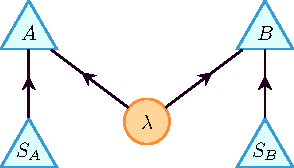
\includegraphics{figure_bell_structure.pdf}}
        \caption{The Bell structure consisting of two observers $A, B$ together with measurement settings $S_{A}$ and $S_{B}$ respectively. The shared latent variable is labeled $\la$.}
        \label{fig:bell_structure}
    \end{figure}


    %\begin{align*}
    %\eq \label{eq:fritz_dist_bit_variant}
    %\begin{split}
    %    \prob[\fritz][00,00,00] = \prob[\fritz][01,01,00] = \prob[\fritz][00,10,01] = \prob[\fritz][01,11,01] &= \f{1}{32}\br{2 + \sqrt{2}} \\
    %    \prob[\fritz][10,00,10] = \prob[\fritz][11,01,10] = \prob[\fritz][10,11,11] = \prob[\fritz][11,10,11] &= \f{1}{32}\br{2 + \sqrt{2}} \\
    %    \prob[\fritz][00,01,00] = \prob[\fritz][01,00,00] = \prob[\fritz][00,11,01] = \prob[\fritz][01,10,01] &= \f{1}{32}\br{2 - \sqrt{2}} \\
    %    \prob[\fritz][10,01,10] = \prob[\fritz][11,00,10] = \prob[\fritz][10,10,11] = \prob[\fritz][11,11,11] &= \f{1}{32}\br{2 - \sqrt{2}}
    %\end{split}
    %\end{align*}


    \begin{acknowledgments}
        The authors would like to thank Rafael Chaves for identifying the error with the wagon-wheel inequality found in earlier versions of this paper.
    \end{acknowledgments}

    % \bibliographystyle{apsrev4-1}
    %\nocite{apsrev41Control}
    %\bibliography{references}

\end{document}
